% Created by tikzDevice version 0.12.6 on 2026-05-17 11:17:00
% !TEX encoding = UTF-8 Unicode
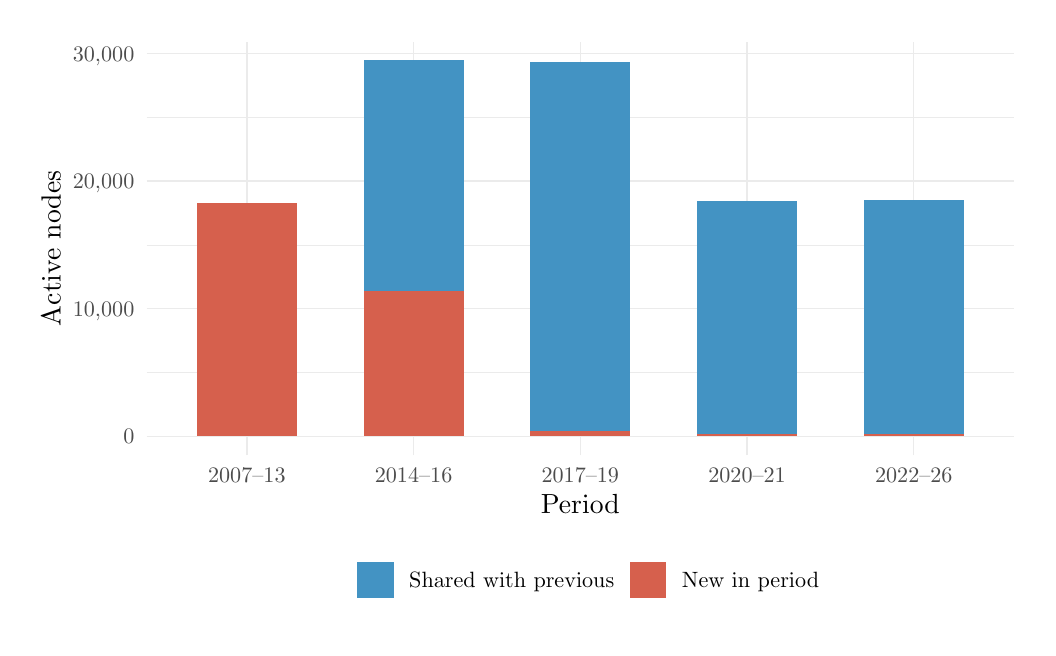
\begin{tikzpicture}[x=1pt,y=1pt]
\definecolor{fillColor}{RGB}{255,255,255}
\path[use as bounding box,fill=fillColor,fill opacity=0.00] (0,0) rectangle (361.35,216.81);
\begin{scope}
\path[clip] (  0.00,  0.00) rectangle (361.35,216.81);
\definecolor{fillColor}{RGB}{255,255,255}

\path[fill=fillColor] ( -0.00,  0.00) rectangle (361.35,216.81);
\end{scope}
\begin{scope}
\path[clip] ( 43.05, 62.35) rectangle (356.35,211.81);
\definecolor{drawColor}{gray}{0.92}

\path[draw=drawColor,line width= 0.3pt,line join=round] ( 43.05, 92.19) --
	(356.35, 92.19);

\path[draw=drawColor,line width= 0.3pt,line join=round] ( 43.05,138.29) --
	(356.35,138.29);

\path[draw=drawColor,line width= 0.3pt,line join=round] ( 43.05,184.38) --
	(356.35,184.38);

\path[draw=drawColor,line width= 0.5pt,line join=round] ( 43.05, 69.14) --
	(356.35, 69.14);

\path[draw=drawColor,line width= 0.5pt,line join=round] ( 43.05,115.24) --
	(356.35,115.24);

\path[draw=drawColor,line width= 0.5pt,line join=round] ( 43.05,161.34) --
	(356.35,161.34);

\path[draw=drawColor,line width= 0.5pt,line join=round] ( 43.05,207.43) --
	(356.35,207.43);

\path[draw=drawColor,line width= 0.5pt,line join=round] ( 79.20, 62.35) --
	( 79.20,211.81);

\path[draw=drawColor,line width= 0.5pt,line join=round] (139.45, 62.35) --
	(139.45,211.81);

\path[draw=drawColor,line width= 0.5pt,line join=round] (199.70, 62.35) --
	(199.70,211.81);

\path[draw=drawColor,line width= 0.5pt,line join=round] (259.95, 62.35) --
	(259.95,211.81);

\path[draw=drawColor,line width= 0.5pt,line join=round] (320.20, 62.35) --
	(320.20,211.81);
\definecolor{fillColor}{RGB}{214,96,77}

\path[fill=fillColor] ( 61.12, 69.14) rectangle ( 97.27,153.33);
\definecolor{fillColor}{RGB}{67,147,195}

\path[fill=fillColor] (121.37,121.61) rectangle (157.52,205.02);
\definecolor{fillColor}{RGB}{214,96,77}

\path[fill=fillColor] (121.37, 69.14) rectangle (157.52,121.61);
\definecolor{fillColor}{RGB}{67,147,195}

\path[fill=fillColor] (181.62, 70.93) rectangle (217.77,204.56);
\definecolor{fillColor}{RGB}{214,96,77}

\path[fill=fillColor] (181.62, 69.14) rectangle (217.77, 70.93);
\definecolor{fillColor}{RGB}{67,147,195}

\path[fill=fillColor] (241.87, 69.89) rectangle (278.02,154.32);
\definecolor{fillColor}{RGB}{214,96,77}

\path[fill=fillColor] (241.87, 69.14) rectangle (278.02, 69.89);
\definecolor{fillColor}{RGB}{67,147,195}

\path[fill=fillColor] (302.12, 70.04) rectangle (338.27,154.57);
\definecolor{fillColor}{RGB}{214,96,77}

\path[fill=fillColor] (302.12, 69.14) rectangle (338.27, 70.04);
\end{scope}
\begin{scope}
\path[clip] (  0.00,  0.00) rectangle (361.35,216.81);
\definecolor{drawColor}{gray}{0.30}

\node[text=drawColor,anchor=base east,inner sep=0pt, outer sep=0pt, scale=  0.80] at ( 38.55, 66.39) {     0};

\node[text=drawColor,anchor=base east,inner sep=0pt, outer sep=0pt, scale=  0.80] at ( 38.55,112.48) {10,000};

\node[text=drawColor,anchor=base east,inner sep=0pt, outer sep=0pt, scale=  0.80] at ( 38.55,158.58) {20,000};

\node[text=drawColor,anchor=base east,inner sep=0pt, outer sep=0pt, scale=  0.80] at ( 38.55,204.68) {30,000};
\end{scope}
\begin{scope}
\path[clip] (  0.00,  0.00) rectangle (361.35,216.81);
\definecolor{drawColor}{gray}{0.30}

\node[text=drawColor,anchor=base,inner sep=0pt, outer sep=0pt, scale=  0.80] at ( 79.20, 52.34) {2007--13};

\node[text=drawColor,anchor=base,inner sep=0pt, outer sep=0pt, scale=  0.80] at (139.45, 52.34) {2014--16};

\node[text=drawColor,anchor=base,inner sep=0pt, outer sep=0pt, scale=  0.80] at (199.70, 52.34) {2017--19};

\node[text=drawColor,anchor=base,inner sep=0pt, outer sep=0pt, scale=  0.80] at (259.95, 52.34) {2020--21};

\node[text=drawColor,anchor=base,inner sep=0pt, outer sep=0pt, scale=  0.80] at (320.20, 52.34) {2022--26};
\end{scope}
\begin{scope}
\path[clip] (  0.00,  0.00) rectangle (361.35,216.81);
\definecolor{drawColor}{RGB}{0,0,0}

\node[text=drawColor,anchor=base,inner sep=0pt, outer sep=0pt, scale=  1.00] at (199.70, 41.40) {Period};
\end{scope}
\begin{scope}
\path[clip] (  0.00,  0.00) rectangle (361.35,216.81);
\definecolor{drawColor}{RGB}{0,0,0}

\node[text=drawColor,rotate= 90.00,anchor=base,inner sep=0pt, outer sep=0pt, scale=  1.00] at ( 11.89,137.08) {Active nodes};
\end{scope}
\begin{scope}
\path[clip] (  0.00,  0.00) rectangle (361.35,216.81);
\definecolor{fillColor}{RGB}{67,147,195}

\path[fill=fillColor] (119.07, 10.65) rectangle (132.23, 23.81);
\end{scope}
\begin{scope}
\path[clip] (  0.00,  0.00) rectangle (361.35,216.81);
\definecolor{fillColor}{RGB}{214,96,77}

\path[fill=fillColor] (217.60, 10.65) rectangle (230.76, 23.81);
\end{scope}
\begin{scope}
\path[clip] (  0.00,  0.00) rectangle (361.35,216.81);
\definecolor{drawColor}{RGB}{0,0,0}

\node[text=drawColor,anchor=base west,inner sep=0pt, outer sep=0pt, scale=  0.80] at (137.88, 14.47) {Shared with previous};
\end{scope}
\begin{scope}
\path[clip] (  0.00,  0.00) rectangle (361.35,216.81);
\definecolor{drawColor}{RGB}{0,0,0}

\node[text=drawColor,anchor=base west,inner sep=0pt, outer sep=0pt, scale=  0.80] at (236.41, 14.47) {New in period};
\end{scope}
\end{tikzpicture}
